\documentclass[conference]{IEEEtran}
\IEEEoverridecommandlockouts
% The preceding line is only needed to identify funding in the first footnote. If that is unneeded, please comment it out.
\usepackage{cite}
\usepackage{amsmath,amssymb,amsfonts}
\usepackage{algorithmic}
\usepackage{graphicx}
\usepackage{textcomp}
\usepackage{xcolor}
\usepackage{float}
\def\BibTeX{{\rm B\kern-.05em{\sc i\kern-.025em b}\kern-.08em
    T\kern-.1667em\lower.7ex\hbox{E}\kern-.125emX}}
\begin{document}

\title{HOMEWOEK 1}

\author{\IEEEauthorblockN{Runlin Hou}
\IEEEauthorblockA{\textit{ECE, School Of Graduate Studies} \\
\textit{Rutgers University}\\
hourunlinxa@gmail.com}
}

\maketitle

\section*{problem 1}
According to the data, the three points with the smallest L2 distance to test data is.
\[\begin{aligned}
    L2_{A1}&=\sqrt{(0-1)^2+(1-0)^2+(1-1)^2}=\sqrt{2}\\
    L2_{C2}&=\sqrt{(0-1)^2+(-1-0)^2+(1-1)^2}=\sqrt{2}\\
    L2_{A0}&=\sqrt{(0-1)^2+(1-0)^2+(0-1)^2}=\sqrt{3}
\end{aligned}\]
When $K=1$, the point chose to decide the class of the test data might be A1 or C2. So 
test data might be classified to be A or C in a same probability. \\
When $K=2$, the points chose to dicide the class of the test data would be A1 and C2,
which means test data got the same probability to be classified in A and C.\\
When $K=3$, all the three points would be chose to decide the class of test data. So the
test data would be classified to be A.

\section*{problem 2}
In this problem, we are supposed to use the KNN to classify
the data into 4 classes -- $[0,1,2,3]$

And the following picture shows the distribution of the 
training data and test data. As we can see, the stars 
are the test data predicted by the model we established
and the dots are the training data.

\begin{figure}[H]
    \centerline{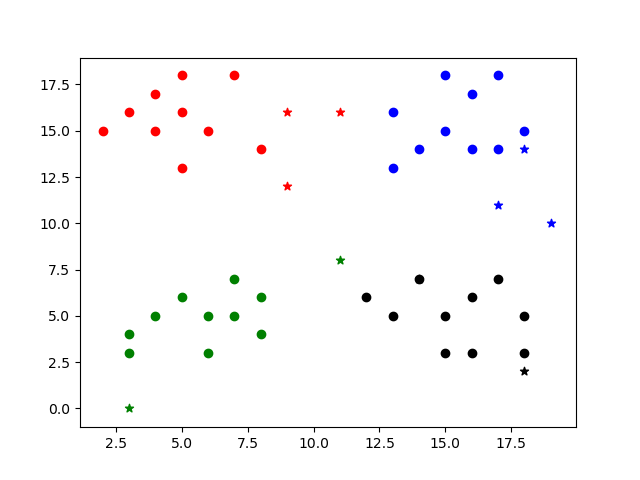
\includegraphics[scale=0.5]{Pic/miniknn.png}}
    \caption{miniKNN}
\end{figure}

\section*{problem 3}
In this section, the data we accepted is a $28\times 28$ image.
To accomplish the training process, we need to do convert the
images into one dimensional array. Here I use \verb|append()|
to merge the 28 row into an array with 784 attributes.

And the trainning process can be achieved with the same code 
from problem 2.

As we can see, I choose the data from 600 to 630 and I finally
achieve an accuracy of $97\%$. The whole process took about 10
seconds.

\begin{figure}[H]
    \centerline{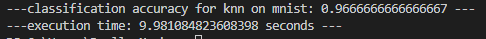
\includegraphics[scale=0.7]{Pic/knn.png}}
    \caption{KNN}
\end{figure}


\end{document}